\documentclass[tikz, border=0mm]{standalone}
\usepackage{ytableau}
\usetikzlibrary{calc}

\newcommand{\tikzsetnextfilename}[1]{}

\newcommand{\ww}[1]{\texttt{#1}}

% Define separation units for layout consistency
\def\xsep{1.5} % Horizontal node separation
\def\ysep{1.5} % Vertical rank separation
% Define the maximum plot width reference (used for justification)
\def\XMax{3.0}


% --- Define Edge Styles ---
\tikzset{
    e1/.style={draw=black, ->, >=stealth, line width=1.2pt},
    e2/.style={draw=black,dashed, ->, >=stealth, line width=1.2pt}
}
\ytableausetup{boxsize=0.9em}

\begin{document}

\tikzsetnextfilename{wordCrystal}
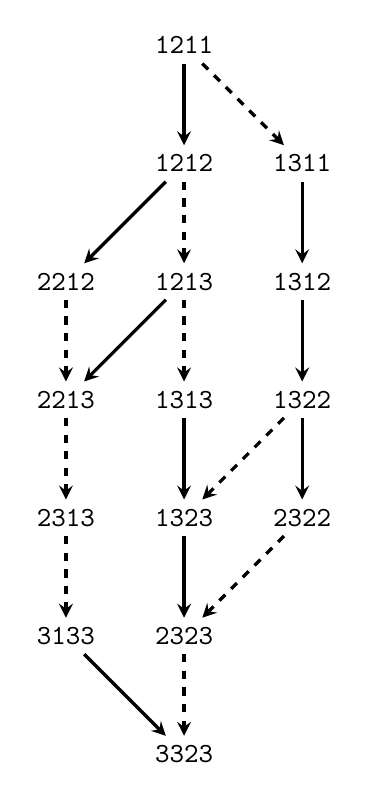
\begin{tikzpicture}[xscale=1.0, yscale=1.0]

% Rank 1 (C=1, Y=9.0, Right-Justified)
\node (R1N1) at (0, 9.0) {\ww{1211}};

% Rank 2 (C=2, Y=7.5, Right-Justified)
\node (R2N1) at (0, 7.5) {\ww{1212}};
\node (R2N2) at (1.5, 7.5) {\ww{1311}};

% Rank 3 (C=3, Y=6.0, Center-Justified)
% X-coords: -1.5, 0.0, 1.5 (Symmetric around X=0)
\node (R3N1) at (-1.5, 6.0) {\ww{2212}};
\node (R3N2) at (0.0, 6.0) {\ww{1213}};
\node (R3N3) at (1.5, 6.0) {\ww{1312}};

% Rank 4 (C=3, Y=4.5, Center-Justified)
\node (R4N1) at (-1.5, 4.5) {\ww{2213}};
\node (R4N2) at (0.0, 4.5) {\ww{1313}};
\node (R4N3) at (1.5, 4.5) {\ww{1322}};

% Rank 5 (C=3, Y=3.0, Center-Justified)
\node (R5N1) at (-1.5, 3.0) {\ww{2313}};
\node (R5N2) at (0.0, 3.0) {\ww{1323}};
\node (R5N3) at (1.5, 3.0) {\ww{2322}};

% Rank 6 (C=2, Y=1.5, Left-Justified)
\node (R6N1) at (-1.5, 1.5) {\ww{3133}};
\node (R6N2) at (0.0, 1.5) {\ww{2323}};

% Rank 7 (C=1, Y=0.0, Left-Justified)
\node (R7N1) at (0, 0.0) {\ww{3323}};

% Rank 1 -> 2
\draw[e1] (R1N1) -- (R2N1);
\draw[e2] (R1N1) -- (R2N2);

% Rank 2 -> 3
\draw[e1] (R2N1) -- (R3N1);
\draw[e2] (R2N1) -- (R3N2);
\draw[e1] (R2N2) -- (R3N3);

% Rank 3 -> 4
\draw[e2] (R3N1) -- (R4N1);
\draw[e1] (R3N2) -- (R4N1);
\draw[e2] (R3N2) -- (R4N2);
\draw[e1] (R3N3) -- (R4N3);

% Rank 4 -> 5
\draw[e2] (R4N1) -- (R5N1);
\draw[e1] (R4N2) -- (R5N2);
\draw[e1] (R4N3) -- (R5N3);
\draw[e2] (R4N3) -- (R5N2);

% Rank 5 -> 6
\draw[e2] (R5N1) -- (R6N1);
\draw[e1] (R5N2) -- (R6N2);
\draw[e2] (R5N3) -- (R6N2);

% Rank 6 -> 7
\draw[e2] (R6N2) -- (R7N1);
\draw[e1] (R6N1) -- (R7N1);

\end{tikzpicture}



\tikzsetnextfilename{ssytCrystal}
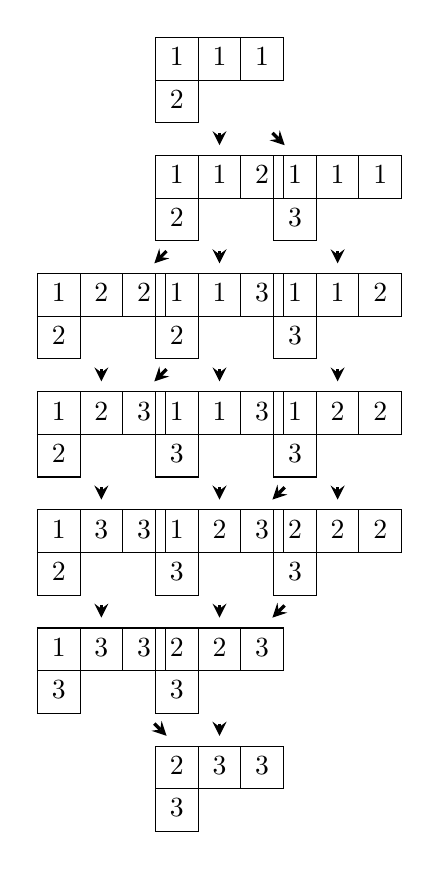
\begin{tikzpicture}[xscale=1.0, yscale=1.0]

% Rank 1 (C=1, Y=9.0, Right-Justified)
\node (R1N1) at (0, 9.0) {\ytableaushort{111,2}};

% Rank 2 (C=2, Y=7.5, Right-Justified)
\node (R2N1) at (0, 7.5) {\ytableaushort{112,2}};
\node (R2N2) at (1.5, 7.5) {\ytableaushort{111,3}};

% Rank 3 (C=3, Y=6.0, Center-Justified)
% X-coords: -1.5, 0.0, 1.5 (Symmetric around X=0)
\node (R3N1) at (-1.5, 6.0) {\ytableaushort{122,2}};
\node (R3N2) at (0.0, 6.0) {\ytableaushort{113,2}};
\node (R3N3) at (1.5, 6.0) {\ytableaushort{112,3}};

% Rank 4 (C=3, Y=4.5, Center-Justified)
\node (R4N1) at (-1.5, 4.5) {\ytableaushort{123,2}};
\node (R4N2) at (0.0, 4.5) {\ytableaushort{113,3}};
\node (R4N3) at (1.5, 4.5) {\ytableaushort{122,3}};

% Rank 5 (C=3, Y=3.0, Center-Justified)
\node (R5N1) at (-1.5, 3.0) {\ytableaushort{133,2}};
\node (R5N2) at (0.0, 3.0) {\ytableaushort{123,3}};
\node (R5N3) at (1.5, 3.0) {\ytableaushort{222,3}};

% Rank 6 (C=2, Y=1.5, Left-Justified)
% X-coords: -1.5, 0.0 (Aligns the leftmost node R6N1 with the central group R3/4/5)
\node (R6N1) at (-1.5, 1.5) {\ytableaushort{133,3}};
\node (R6N2) at (0.0, 1.5) {\ytableaushort{223,3}};

% Rank 7 (C=1, Y=0.0, Left-Justified)
\node (R7N1) at (0, 0.0) {\ytableaushort{233,3}};

% Rank 1 -> 2
\draw[e1] (R1N1) -- (R2N1);
\draw[e2] (R1N1) -- (R2N2);

% Rank 2 -> 3
\draw[e1] (R2N1) -- (R3N1);
\draw[e2] (R2N1) -- (R3N2);
\draw[e1] (R2N2) -- (R3N3);

% Rank 3 -> 4
\draw[e2] (R3N1) -- (R4N1);
\draw[e1] (R3N2) -- (R4N1);
\draw[e2] (R3N2) -- (R4N2);
\draw[e1] (R3N3) -- (R4N3);

% Rank 4 -> 5
\draw[e2] (R4N1) -- (R5N1);
\draw[e1] (R4N2) -- (R5N2);
\draw[e1] (R4N3) -- (R5N3);
\draw[e2] (R4N3) -- (R5N2);

% Rank 5 -> 6
\draw[e2] (R5N1) -- (R6N1);
\draw[e1] (R5N2) -- (R6N2);
\draw[e2] (R5N3) -- (R6N2);

% Rank 6 -> 7
\draw[e2] (R6N2) -- (R7N1);
\draw[e1] (R6N1) -- (R7N1);

\end{tikzpicture}




\end{document}
